\chapter{Results}
\label{chapter:results}

As mentioned in section \ref{section:intro-contributions}, at the core of our thesis are three experiments whose goal is to evaluate our method, show results that have not been achieved with conventional per-pixel projection mapping methods and show that statistics-based projection mapping is worth pursuing further.

In this chapter, we guide the reader through each experiment, first explaining its goal, hypothesis and setup, then showing the results and finally providing an analysis.

{\color{red} TODO: mention that analysis is only subjective and relies on visual inspection!}

\section{Evaluating basic rendering function and basic texture model together}
\label{section:results-experiments-01}

The basic idea of our proposed method is that when projecting a texture, is that instead of mapping it directly, we use a texture synthesis algorithm to generate another example of the same texture so that it is easier to map than the original texture. Assuming our texture model is good and we are able to push it to generate textures that are easy to map, our method is better than conventional pixel-based projection mapping methods (when projecting textures).

\textbf{Goal.} In the first experiment, the goal is to find out whether our method is indeed able to push the synthesis algorithm to generate textures that map well onto a given scene.

\textbf{Hypothesis}. We consider a simple projection scenario described in section \ref{section:methods-rendering_function-simple}. Next, we set our background to be a subset of the input texture. If our method works as expected, it will generate an image which has white pixels where the background matches the texture and continue organically around this area. This is because such a solution is that of least effort.

\textbf{Setup.} In our pipeline, we use the simple rendering function (see \ref{section:methods-rendering_function-simple}) because it is sufficient to reproduce the conditions of our experiment. We will also use the original unmodified Gatys texture model (see \ref{section:methods-texture_model}) because we are not interested in overall performance, but simply whether it is possible to add restrictions to the texture model to make it generate only textures that match the background. The inputs to this experiment are pairs of scene (represented by a background image) and texture image that we wish to project-map.

\subsection{Results}
\label{section:results-experiments-01-results}

\begin{figure}[ht]
    \begin{center}
        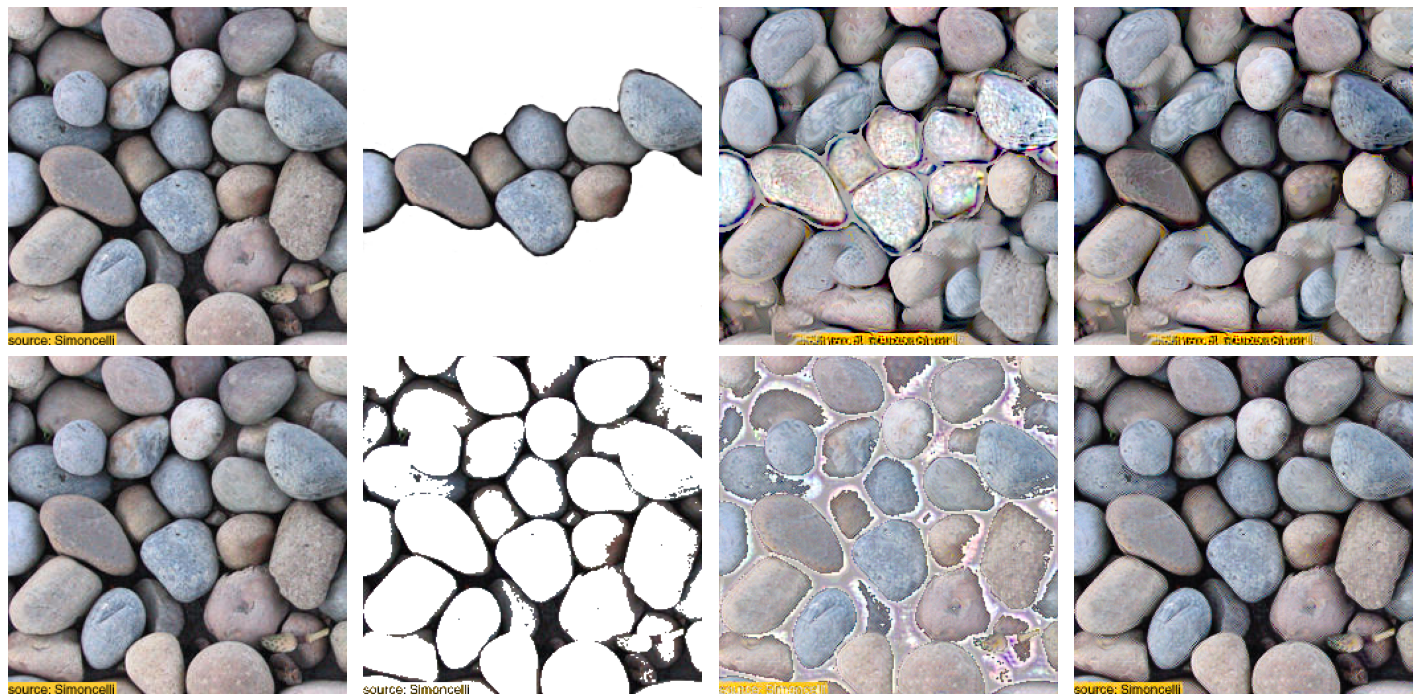
\includegraphics[width=0.8\textwidth]{images/ex01-pebbles-1000steps-crop.png}
        \caption{{\color{red} TODO: texture source? self-contained description! better figure!}}
        \label{fig:ex01-pebbles-1000steps}
    \end{center}
\end{figure}

Figure \ref{fig:ex01-pebbles-1000steps} shows the main result of this experiment. Overall, we have tested five different backgrounds and two different input texture. Complete results of those runs can be found in the appendix \ref{chapter:appendix-results}.

\subsection{Analysis}
\label{section:results-experiments-01-analysis}

\begin{figure}[ht]
    \begin{center}
        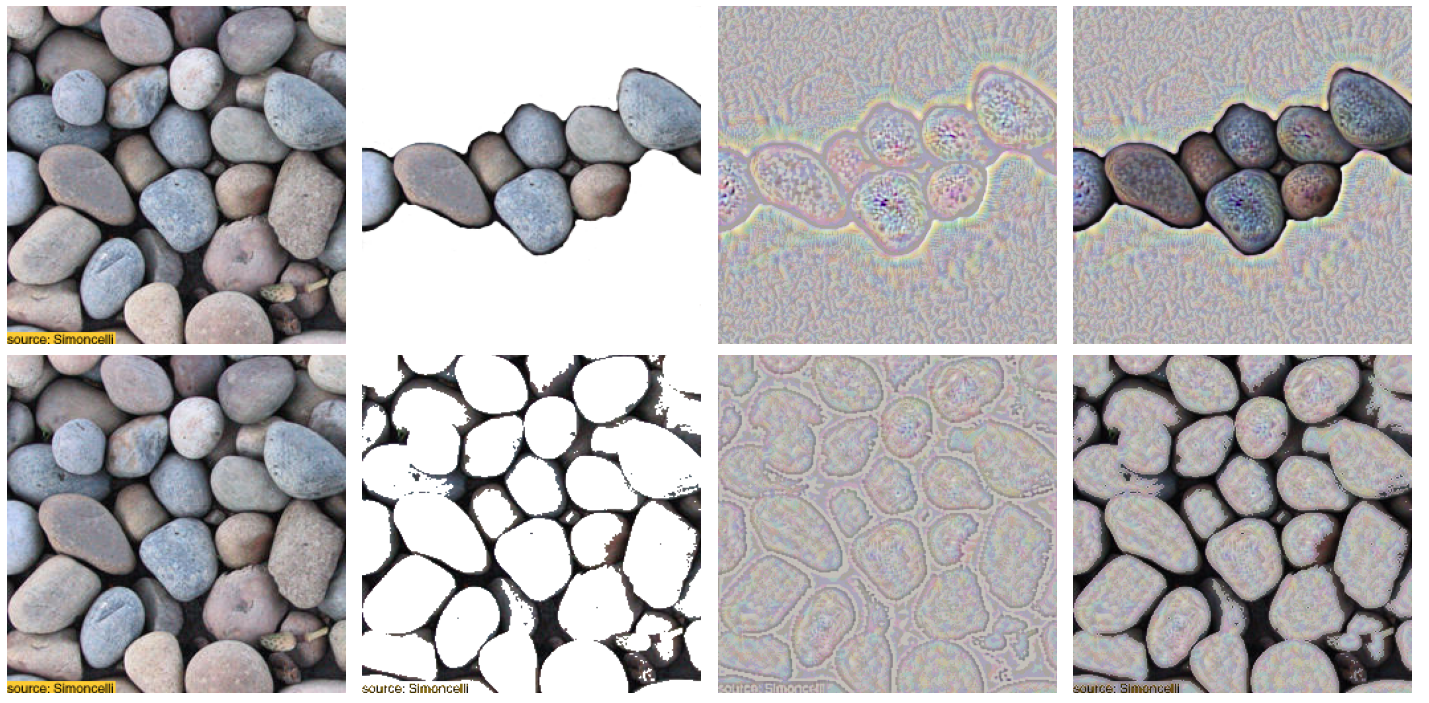
\includegraphics[width=0.8\textwidth]{images/ex01-pebbles-5steps-crop.png}
        \caption{{\color{red} TODO: texture source? self-contained description! better figure!}}
        \label{fig:ex01-pebbles-5steps}
    \end{center}
\end{figure}

It can be said that our method is indeed capable of controlling the synthesis in a way that yields those textures that match the background well. The algorithm largely respects the texture features which are already present in the background and continues the texture smoothly around them. 

Especially interesting is the second row in figure \ref{fig:ex01-pebbles-1000steps} where the outlines of all the pebbles are fixed by the background. Our method not only respects those boundaries, but also reproduces the input texture almost perfectly. This means that the second background restricts the Gatys texture model much more than the first background. ({\color{red} TODO: analyze a bit more -- micro vs. macro features, some literature, \dots})

On the other hand, in the first row of figure \ref{fig:ex01-pebbles-1000steps}, we can see that the area where the background matches the input is not fully saturated as expected. A possible explanation for this is that the algorithm starts from a white noise image with mean \(0.5\) (see figure \ref{fig:ex01-pebbles-5steps}). Combined with the fact that the loss decreases the fastest at the beginning of the optimization process ({\color{red} TODO: graph?}), this likely translated into the algorithm prefering to leave the middle area of the image darker and compensating overall brightness by making the surrounding pebbles brighter, rather than matching the exact appearance of the middle area to that of the input. From the perspective of this experiment, however, this is not a major issue.

\section{Evaluating various texture models}
\label{section:results-experiments-02}

{\color{red} TODO: use the notes from OrgPad, they look pretty good an even have some nice ideas for further analysis!}

% \textbf{Goal:} To project-map textures better than per-pixel algorithms can in certain scenarios. \textbf{Method:} We try various texture models in our method, comparing them to a per-pixel reference algorithm. \textbf{Question:} Will our method perform better by adapting the texture to fit the background and therefore hiding it more effectively?

% We keep using the simplified rendering function in the second experiment as well. We would like to know whether our method lives up to the theoretical promise of better perormance in challenging situations compared to pixel-based projection mapping approaches. And these situations can also be reproduced in the simplified scenario because we are mostly interested in cases where the projector would be forced out of its color gamut by a pixel-based projection mapping algorithm. In the simplified scenario, this happens for example when we want to project a bright pixel onto a dark patch of the background.

% Here are our pairs of scene and background for this experiment:

% {\color{red} TODO: insert image pairs here}

% First, we want to compare the performance of our method to a reference pixel-based method. We obtain the reference pixel-based method by removing the texture model block from out pipeline and replacing it with a per-pixel L2 difference between the input texture image and the optimized image. This approach yields the optimal pixel-based projection mapping algorithm without a content-based global optimization step (as described in section \ref{section:background-projection_mapping-procams-radiometric_calibration}). ({\color{red} TODO: why leave the global step out?}).

% Within our method, we also want to compare the performance of the original Gatys texture model with one that incorporates improvements described in section \ref{section:methods-texture_model-improvements}.

% The expectation is that our method will outperform the pixel-based reference in challenging areas of the scene by moving dark texture features into dark areas of the background and vice-versa. As a result, the background should be less recognizable when projected onto with our optimized projection image. As far as various texture models are concerned, we expect the Gatys model to adapt to the background more because its texture description is less constrained. Other than that, the question is whether the improvements bring better results in projection mapping as they do in pure texture synthesis.

\section{Evaluating complex rendering function}
\label{section:results-experiments-03}

% \textbf{Goal:} To have a rendering function that simulates a projector accurately in all possible scenarios. \textbf{Method:} Projection mapping onto arbitrary 3D scenes with our method, as well as the per-pixel reference. \textbf{Question:} Will behaviour from experiment 2 translate well into this more complex scenario?

% So far we have only used the simplified rendering function which projects images into a flat diffuse background. The last question we will focus on here is whether the observations from the previous experiment (\ref{section:methods-experiments-02}) will also apply when projecting onto arbitrary 3D scenes. We have chosen the following textures and scenes from this experiment:

% {\color{red} TODO: insert textures and scenes here and explain the scenes well}

% As mentioned in section \ref{section:methods-rendering_function-complex-lt_capture}, our implementation of the complex rendering function only handles fairly small image resolutions. However, as can be seen from the figure above, even \(160 \times 160\) images should be sufficient to model the conditions from the previous experiment and we thus expect the behaviour to translate as well.